\documentclass[tikz,border=2pt]{standalone}
\usepackage{amsmath}
\usetikzlibrary{arrows.meta}
\begin{document}
% Battle of the Sexes: player 1 (rows, blue) marks the best payoff in each column,
% player 2 (columns, red) marks the best payoff in each row; the doubly marked cells
% (O,O) and (F,F) are the two pure Nash equilibria.
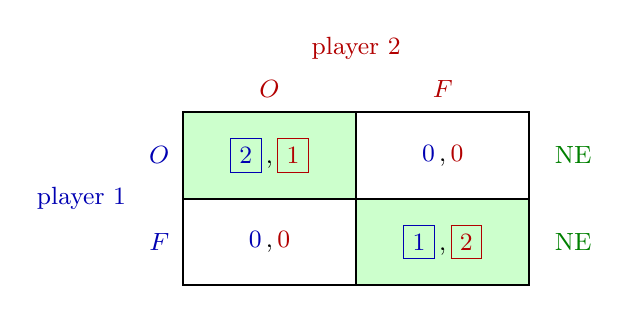
\begin{tikzpicture}[font=\small, >={Latex[length=2mm]}]
  \def\w{2.2} \def\h{1.1}
  % equilibrium cells
  \fill[green!20] (0,0) rectangle (\w,\h);
  \fill[green!20] (\w,-\h) rectangle (2*\w,0);
  \draw[thick] (0,-\h) rectangle (2*\w,\h);
  \draw[thick] (\w,-\h) -- (\w,\h);
  \draw[thick] (0,0) -- (2*\w,0);
  % strategy labels
  \node[red!70!black] at (0.5*\w,\h+0.3) {$O$};
  \node[red!70!black] at (1.5*\w,\h+0.3) {$F$};
  \node[blue!70!black] at (-0.3,0.5*\h) {$O$};
  \node[blue!70!black] at (-0.3,-0.5*\h) {$F$};
  \node[red!70!black, anchor=south] at (\w,\h+0.55) {player 2};
  \node[blue!70!black, anchor=east] at (-0.6,0) {player 1};
  % payoffs (marked best responses boxed)
  \node at (0.5*\w,0.5*\h) {\textcolor{blue!70!black}{$\boxed{2}$}\,,\,\textcolor{red!70!black}{$\boxed{1}$}};
  \node at (1.5*\w,0.5*\h) {\textcolor{blue!70!black}{$0$}\,,\,\textcolor{red!70!black}{$0$}};
  \node at (0.5*\w,-0.5*\h) {\textcolor{blue!70!black}{$0$}\,,\,\textcolor{red!70!black}{$0$}};
  \node at (1.5*\w,-0.5*\h) {\textcolor{blue!70!black}{$\boxed{1}$}\,,\,\textcolor{red!70!black}{$\boxed{2}$}};
  % legend-free note
  \node[green!50!black, anchor=west] at (2*\w+0.2,0.5*\h) {NE};
  \node[green!50!black, anchor=west] at (2*\w+0.2,-0.5*\h) {NE};
\end{tikzpicture}
\end{document}
